\documentclass[a4paper,11pt]{report}
\usepackage{a4wide}
\usepackage[english]{babel}
\usepackage{graphicx,subfigure}
\setcounter{secnumdepth}{3} 


\author{Cedric~Cuypers, Kenzo~Tomita, Guy~Van~den~Broeck} 
% define title
\title{Security Requirements: Poker Application} 

\bibliographystyle{alpha}

\begin{document} 
% generates the title 
\maketitle 
% insert the table of contents 
\tableofcontents 

\chapter{Introduction}
This document starts from an existing architecture of a poker application that was originally designed with only an intuitive idea of security threats for poker applications. By modelling the data flow through the application we try to locate areas that can be subjected to these threats. 

For a subset of entities we apply STRIDE to elicit security threats and we use threat tree patterns to render these threats more concrete. The results are documented as misuse cases.

Finally, we present examples of business threats that cannot be discovered using the STRIDE methodology. 


\chapter{Identifying threats}
\section{DFDs}
Figure \ref{fig:context} shows the context level of the DFD. Figure \ref{fig:level_0} shows the level-0 DFD. The arrows are not annotated to make the diagram readable. A simplified version with only the player and annotated arrows can be found in figure \ref{fig:level_0_player}. In the following analysis only the interaction with the player will be considered as misuse cases, as those with an administrator as external entity are similar. Although some processes are complex and should be drilled down, we've chosen to do the STRIDE analysis on level-0 because it would already generate sufficient documentation.

There are several trust boundaries that can be identified in the DFDs. First of all there is the trust boundary between the external entities and the processes. All input coming from the external entities should be validated and the data flow from the processes to the external entities should be analyzed for not leaking sensitive, private or confidential data. Inside this trust boundary several smaller trust boundaries can be recognized. These are the processes that deal with sensitive, private data: 
\begin{itemize}
\item \textbf{Account Management:} account data should be protected and all data flowing out of this process should be verified extensively. 
\item \textbf{Table:} hole cards are confidential data only accessible for the player to whom they belong and the game engine to verify the winner at the end of a deal.
\item \textbf{Logging Engine:} the logging should happen in a secure way so there is no possibility to alter the log, therefor the log entries arriving at the logging engine should be validated. The log also contains very sensitive data, so the access is only allowed to a very limited number of entities and processes.
\end{itemize}
 

\begin{figure}[h]
  \begin{center}
    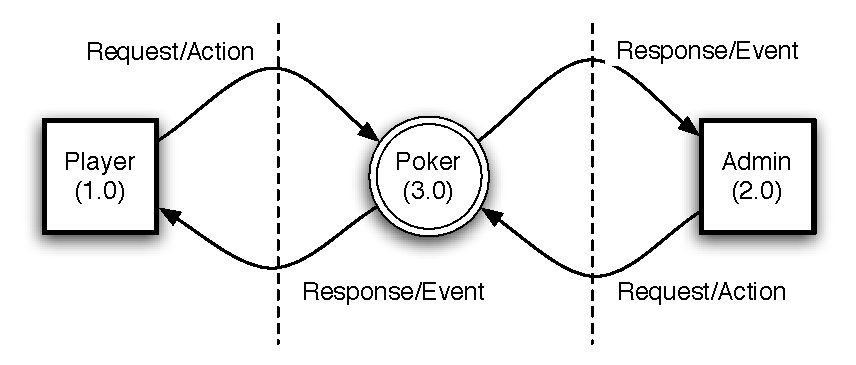
\includegraphics[scale=0.8]{context_diagram}
  \end{center}
  \caption{Context Level DFD}\label{fig:context}
\end{figure}

\begin{figure}[p]
  \begin{center}
    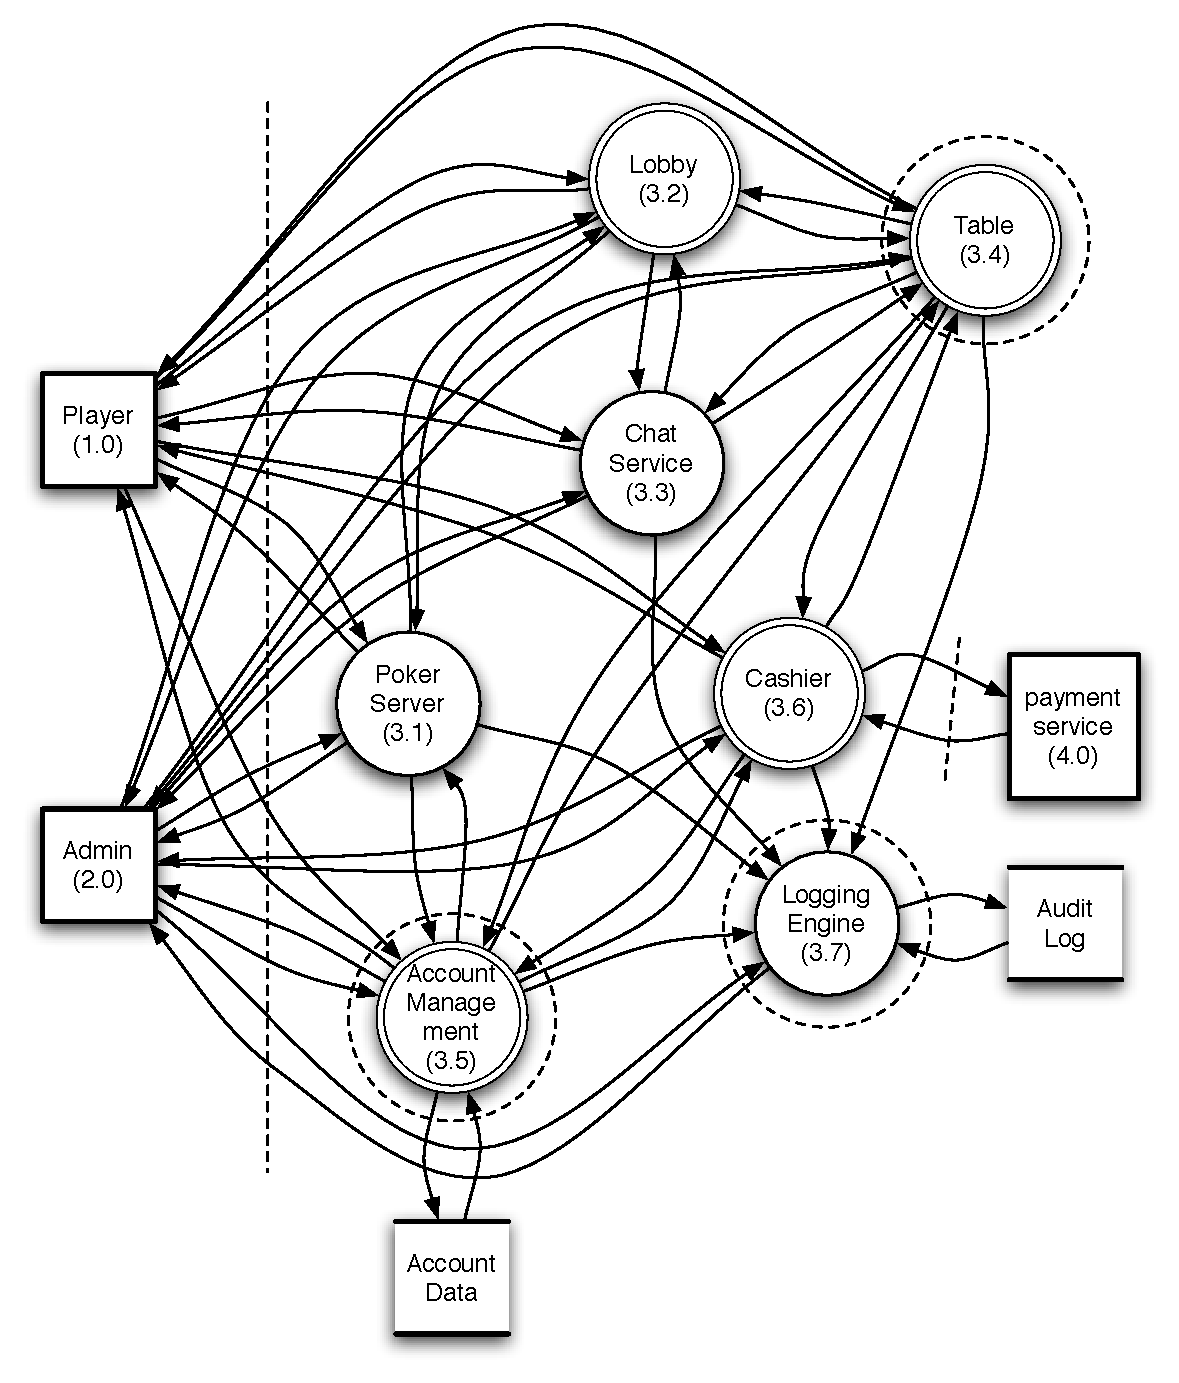
\includegraphics[scale=0.8]{dfd_level_0}
  \end{center}
  \caption{DFD Level-0}\label{fig:level_0}
\end{figure}

\begin{figure}[p]
  \begin{center}
    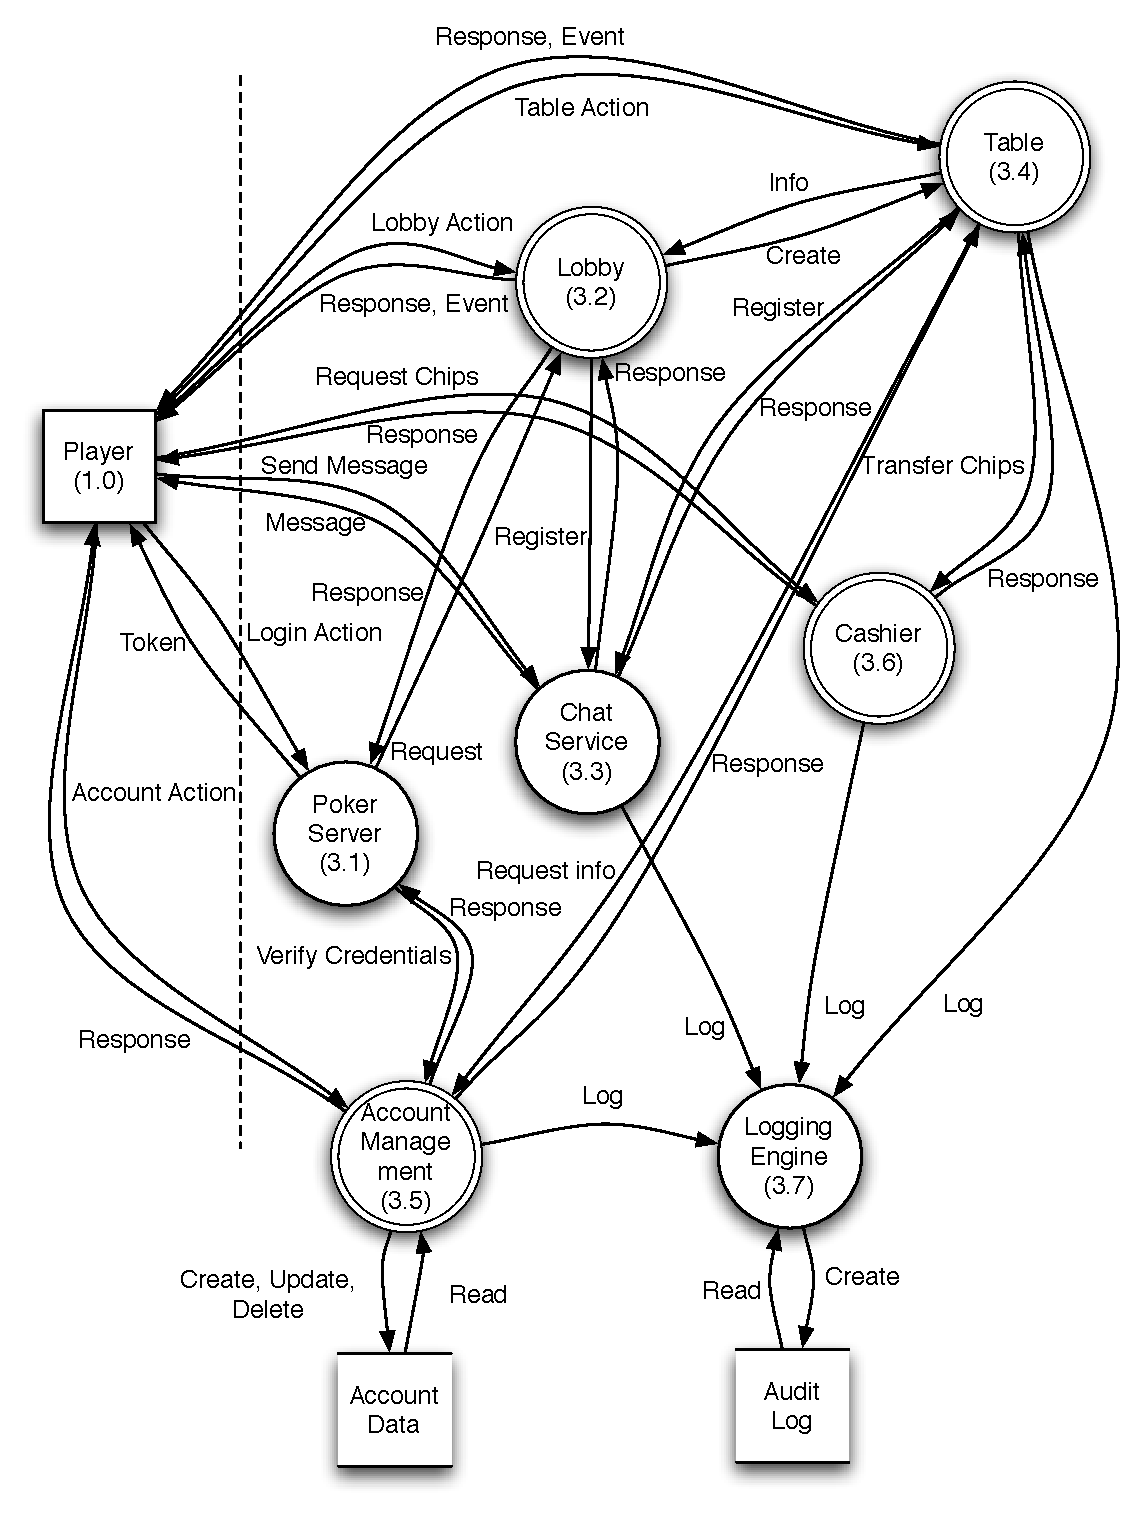
\includegraphics[scale=0.7]{dfd_level_0_player}
  \end{center}
  \caption{DFD Level-0 - only player}\label{fig:level_0_player}
\end{figure}

\section{Rationale}
\subsection{Assumptions}
\begin{itemize}
\item There is an internal policy to restrict physical access to the servers. 
\item There is no protection needed against an administrator with a debugger (can read and alter memory).
\item Side channels aren't available to mis-actors.
\end{itemize}

\section{Architecture based Misuse Cases}
\subsection{Player}
\subsubsection{Spoofing a Player}
\textbf{Summary:} \\
The mis-actor gains access to the poker server pretending to be a legitimate user. To achieve this goal he can use false credentials or credentials of an existing user. He could also bypass the authentication system to realize the same objective. \\
\textbf{Primary mis-actor:}
\begin{itemize}
\item Crook
\end{itemize}
\textbf{Basic path:}
\begin{itemize}
\item The mis-actor obtains the credentials of a legitimate player.
\item The mis-actor authenticates with the poker server.
\item The mis-actor can take actions on behalf of a legitimate player.
\end{itemize}
\textbf{Alternative paths:}
\begin{itemize}
\item The mis-actor bypasses the authentication system by exploiting a weakness.
\item The mis-actor finds a way to fake credentials.
\end{itemize}
\textbf{Capture points:}
\begin{itemize}
\item \textbf{Prevention:}
\begin{itemize}
\item Make sure credentials are well protected on the server side.
\item Transmit credentials over the wire securely.
\item Test credentials for uniqueness and complexity.
\item Certify client software to enforce that credentials are handled securely.
\end{itemize}
\end{itemize}
\textbf{Triggers:}\\
Always true, i.e., this can happen at any time. \\
\textbf{Preconditions:}
\begin{itemize}
\item Credentials can be falsified.
\item Credentials are not well protected.
\item There is no authentication system or the authentication system is too weak.
\end{itemize}
\textbf{Assumptions:}
\begin{itemize}
\item The players are careless with their credentials (e.g. store user name/password in a text file).
\item The players choose easy passwords.
\end{itemize}
\textbf{Worst case threat:}\\
The crook can play with the spoofed identity against his own identity and win all chips from spoofed identity. \\
\textbf{Prevention Guarantee:} \\
Only authentic users can gain access at the poker server. \\
\textbf{Stakeholders and risks:}
\begin{itemize}
\item Player: 
\begin{itemize}
\item Potential loss of money if his identity is misused and all chips are transfered to an other account.
\end{itemize}
\item Online Casino: 
\begin{itemize}
\item Lost confidence if security problems get publicized.
\end{itemize}
\end{itemize}

\subsubsection{Repudiation of a Player}
\label{Repudiation of a Player}
\textbf{Primary mis-actor:}
\begin{itemize}
\item Crook
\end{itemize}
\textbf{Basic path:}
\begin{itemize}
\item The mis-actor performs an action or transaction.
\item The mis-actor repudiates the action or transaction For example, he repudiates his bet when it turns out that another player has a better hand.
\item The system fails to prove that the mis-actor is responsible.
\end{itemize}
\textbf{Alternative paths:}
\begin{itemize}
\item The mis-actor tampers with the logging process to remove evidence.
\end{itemize}
\textbf{Capture points:}
\begin{itemize}
\item \textbf{Prevention:}
\begin{itemize}
\item Use a strong signature system for messages originating from the player.
\item Use antireplay defences.
\item Log all actions and transactions.
\item Secure access to the logging process.
\end{itemize}
\end{itemize}

\subsection{Poker Server}
\subsubsection{Spoofing the poker server}
\textbf{Primary mis-actor:}
\begin{itemize}
\item Crook
\end{itemize}
\textbf{Basic path:}
\begin{itemize}
\item The mis-actor prepares the process that can spoof a poker server.
\item The mis-actor deploys its process on the online casino servers (performed by a skilled insider).
\item The mis-actor can cheat and steal sensitive data from the users.
\end{itemize}
\textbf{Alternative paths:}
\begin{itemize}
\item The mis-actor deploys its process on an external server (performed by a skilled outsider).
\end{itemize}
\textbf{Capture points:}
\begin{itemize}
\item \textbf{Prevention:}
\begin{itemize}
\item Only administrators of the online casino can place code on the online poker servers.
\item Only the code that is running on trusted locations can be used as part of the system.
\item Poker servers are authenticated.
\item Messages coming out of the poker server are signed.
\end{itemize}
\end{itemize}

\subsubsection{Tampering with the poker server}
\textbf{Primary mis-actor:}
\begin{itemize}
\item Crook
\end{itemize}
\textbf{Basic path:}
\begin{itemize}
\item The mis-actor sends invalid input to the poker server.
\item The message corrupts the state of the poker server. 
\item While the poker server is in the corrupted state, the mis-actor controls the behavior of that poker server.
\item The mis-actor can cheat and steal sensitive data from the users.
\end{itemize}
\textbf{Alternative paths:}
\begin{itemize}
\item The mis-actor provides false credentials (spoofing an administrator) and modifies the poker server.
\end{itemize}
\textbf{Capture points:}
\begin{itemize}
\item \textbf{Prevention:}
\begin{itemize}
\item All input is validated.
\item Spoofing an administrator should be impossible.
\end{itemize}
\end{itemize}

\subsubsection{Repudiation of an action at the poker server}
See section \ref{Repudiation of a Player}.

\subsubsection{Information disclosure at the poker server}
\textbf{Primary mis-actor:}
\begin{itemize}
\item Crook
\end{itemize}
\textbf{Basic path:}
\begin{itemize}
\item The mis-actor spoofs another actor with access to private information (e.g. user names, passwords, ...).
\item The mis-actor uses the private information.
\end{itemize}
\textbf{Alternative paths:}
\begin{itemize}
\item Elevation of privilege of the mis-actor leads to information disclosure.
\item The mis-actor sends invalid input to the poker server.
\item The mis-actor has access to the memory and can alter its state (e.g. debugging mode).
\end{itemize}
\textbf{Capture points:}
\begin{itemize}
\item \textbf{Prevention:}
\begin{itemize}
\item All input is validated.
\end{itemize}
\end{itemize}

\subsubsection{DoS against the poker server}
\textbf{Primary mis-actor:}
\begin{itemize}
\item Crook
\end{itemize}
\textbf{Basic path:}
\begin{itemize}
\item The mis-actor sends invalid input to the poker server. 
\item The poker server crashes.
\item The poker server becomes unavailable.
\end{itemize}
\textbf{Alternative paths:}
\begin{itemize}
\item The mis-actor crashes the poker server by tampering with the poker server.
\item The mis-actor consumes application-specific resources (e.g. send more login requests per second than the poker server can handle).
\item The mis-actor consumes fundamental resources.
\end{itemize}
\textbf{Capture points:}
\begin{itemize}
\item \textbf{Prevention:}
\begin{itemize}
\item All input is validated.
\item The poker server is load-balanced.
\end{itemize}
\item \textbf{Detection:}
\begin{itemize}
\item Access to the poker server is securely logged.
\end{itemize}
\end{itemize}

\subsubsection{Elevation of privilege at the poker server}
\textbf{Primary mis-actor:}
\begin{itemize}
\item Crook
\end{itemize}
\textbf{Basic path:}
\begin{itemize}
\item The mis-actor logs in.
\item He activates the role (administrator) with higher privileges.
\item The mis-actor gains higher privileges. 
\item The mis-actor misuses the higher privileges.
\end{itemize}
\textbf{Alternative paths:}
\begin{itemize}
\item The mis-actor spoofs the identity of an other actor (administrator) with higher privileges.
\item The mis-actor tampers with the poker server to gain more privileges. 
\item The mis-actor sends invalid input to the poker server. 
\item The mis-actor has access to the memory and can alter its state (e.g. debugging mode).
\end{itemize}
\textbf{Capture points:}
\begin{itemize}
\item \textbf{Prevention:}
\begin{itemize}
\item Authentication and authorisation system that verifies credentials.
\item Spoofing user and tampering with poker server prevention.
\end{itemize}
\item \textbf{Detection:}
\begin{itemize}
\item Access to the poker server is securely logged. The log can be compared with the security policy to verify if an actor is allowed to do the action.
\end{itemize}
\end{itemize}

\subsection{Lobby}
\subsubsection{Spoofing a lobby}
\textbf{Summary:} \\
The mis-actor prepares a process to spoof the lobby and deploys it on one of the online casino servers or on an external server. Every player connecting to a table through the lobby can be diverted to an untrusted table.
\subsubsection{Tampering with the lobby}
\textbf{Summary:} \\
The mis-actor tampers with the lobby to modify its functionality. A player connecting to a table through the lobby can be diverted to an untrusted table. 
\subsubsection{Repudiation of an action at the lobby}
\subsubsection{Information disclosure at the lobby}
\subsubsection{DoS against the lobby}
\textbf{Summary:} \\
The mis-actor performs actions leading to a crash or overloading the capacity of the lobby. As a result, the lobby can no longer be reached by the users.
\subsubsection{Elevation of privilege at the lobby}
\textbf{Summary:} \\
The mis-actor performs actions leading to the possibility to do administrator actions. He can achieve this by presenting false credentials, spoofing an administrator or tampering with the lobby or account management.
\subsection{Table}
\subsubsection{Spoofing a table}
\textbf{Summary:} \\
The mis-actor prepares a process to spoof the table and deploys it on one of the online casino servers or on an external server. Every player connecting to this table can be scammed. The spoofed table could provide the mis-actor with all confidential information or deal crafted hands to maximize the profit of the mis-actor (e.g. deal a full house to an innocent player and deal a four of a kind to himself and lure the innocent player to go all-in).
\subsubsection{Tampering with a table}
\textbf{Summary:} \\
The mis-actor tampers with the lobby to modify its functionality. Every player connecting to this table can be scammed. The tampered table could provide the mis-actor with all confidential information or deal crafted hands to maximize the profit of the mis-actor (e.g. deal a full house to an innocent player and deal a four of a kind to himself and lure the innocent player to go all-in).
\subsubsection{Repudiation of a table}
\textbf{Summary:} \\
The online casino denies a player has won a number of chips or has received certain hole cards. This is possible if there is no log or if the log could be modified. It is also possible that the hand evaluation system has been tampered and this should be detected afterwards. 
\subsubsection{Information disclosure at a table}
\textbf{Primary mis-actor:}
\begin{itemize}
\item Crook
\end{itemize}
\textbf{Basic path:}
\begin{itemize}
\item The mis-actor spoofs an other actor with access to private information regarding this table
(e.g. pocket cards of players, ...).
\item The mis-actor uses the private information.
\end{itemize}
\textbf{Alternative paths:}
\begin{itemize}
\item Elevation of privilege of the mis-actor leads to information disclosure.
\item The mis-actor sends invalid input to the table.
\item The mis-actor has access to the memory and can alter its state (e.g. debugging mode).
\end{itemize}
\textbf{Capture points:}
\begin{itemize}
\item \textbf{Prevention:}
\begin{itemize}
\item All input is validated.
\end{itemize}
\item \textbf{Detection:}
\begin{itemize}
\item The behavior of the mis-actor is influenced by the information disclosure. This altered behavior could be detected by examining the logs.
\end{itemize}
\end{itemize}

\subsubsection{DoS against a table}
\textbf{Summary:} \\
The mis-actor performs actions leading to a crash or overloading the capacity of the table. As a result, the table can no longer be reached by the users.
\subsubsection{Elevation of Privilege at the table}
\textbf{Summary:} \\
The mis-actor performs actions leading to the possibility to do administrator actions. He can achieve this by presenting false credentials, spoofing an administrator or tampering with the lobby or account management.
\subsection{Chat Service}
\subsection{Cashier}
\subsection{Account Management}
\subsubsection{Spoofing the account management system}
\subsubsection{Tampering with the account management system}
\subsubsection{Repudiation of using the account management system}
\subsubsection{Information disclosure of the account management system}
\subsubsection{DoS against the account management system}
\subsubsection{Elevation of Privilege}
\subsection{Account Data}
\subsubsection{Tampering with account data}
\textbf{Primary mis-actor:}
\begin{itemize}
\item Crook
\end{itemize}
\textbf{Basic path:}
\begin{itemize}
\item The mis-actor gains access to the data store
\item The mis-actor puts data directly in the data store
\end{itemize}
\textbf{Alternative paths:}
\begin{itemize}
\item The mis-actor removes data directly from the data store
\item There may be overcapacity failures: the mis-actor floods the data store by placing large 
amounts of data into the data store. As a consequence data in the beginning of the store might be overwritten
, data written to the store might be discarded or the data store might crash, depending on the implementation of
the data store.
\end{itemize}
\textbf{Capture points:}
\begin{itemize}
\item \textbf{Prevention:}
\begin{itemize}
\item placing and removing of data in the data store is securely logged
\item data store is protected by the internal policies
\item extra-monitor access is impossible (behind a reliable firewall)
\item overcapacity failures are handled accordingly
\item only private or local networks are used for communication between the account management process 
and the account data store.
\end{itemize}
\item \textbf{Detection:}
\begin{itemize}
\item logs can be searched for adding of removing falsified data
\end{itemize}
\end{itemize}

\subsubsection{Information disclosure of account data}
\textbf{Primary mis-actor:}
\begin{itemize}
\item Crook
\end{itemize}
\textbf{Basic path:}
\begin{itemize}
\item The mis-actor gains access to the data store.
\item The mis-actor reads private data from data store.
\end{itemize}
\textbf{Alternative paths:}
\begin{itemize}
\item The mis-actor spoofs the account management process
\end{itemize}
\textbf{Capture points:}
\begin{itemize}
\item \textbf{Prevention:}
\begin{itemize}
\item encrypting the data 
\item data store is protected by the internal policies
\item extra-monitor access is impossible (behind a reliable firewall)
\item only private or local networks are used for communication between the account management process 
and the account data store.
\item prevent spoofing of account management process
\end{itemize}
\end{itemize}

\subsubsection{DoS against account data}
\textbf{Primary mis-actor:}
\begin{itemize}
\item Crook
\end{itemize}
\textbf{Basic path:}
\begin{itemize}
\item The mis-actor gains access to the data store.
\item The mis-actor corrupts the data store by sending invalid input.
\item The data store crashes and becomes unavailable.
\end{itemize}
\textbf{Alternative paths:}
\begin{itemize}
\item The mis-actor floods the data store by placing large amounts of data into the data store and exceeds the 
capacity of the data store.
\item The mis-actor consumes application-specific resources (e.g. submit more queries per second that the data 
store can handle).
\item The mis-actor injects malicious SQL queries (or other) to an user of the data store. When this injection reaches the data store it crashes.
\end{itemize}
\textbf{Capture points:}
\begin{itemize}
\item \textbf{Prevention:}
\begin{itemize}
\item Invalid queries are filtered.
\item Data store is protected by the internal policies.
\item Extra-monitor access is impossible (behind a reliable firewall).
\item Only private or local networks are used for communication between the account management process 
and the account data store.
\item The data store is load-balanced.
\end{itemize}
\end{itemize}
\subsection{Logging Engine}
\subsubsection{Spoofing the logging engine}
\subsubsection{Tampering with the logging engine}
\subsubsection{Repudiation of using the logging engine}
\subsubsection{Information disclosure of the logging engine}
\subsubsection{DoS against the logging engine}
\subsubsection{Elevation of Privilege}
\subsection{Audit Log}
\subsubsection{Tampering with the audit log}
\subsubsection{Repudiation of logging something in the audit log}
\subsubsection{Information disclosure of the audit log}

\subsection{Data Flows from a Player}

According to \cite[p117]{1202957}, one of the first concerns before doing threat analysis should be to reduce the number of entities to analyze.
Here we choose to reduce the number of data flows from/to the Player because interaction between a Player and the different processes is very similar (using the same technology, similar entities with similar confidentiality). We only consider requests for tokens (login actions), actions sent to a process, tokens sent to a Player and events/responses sent to a Player.

\subsubsection{Tampering with token requests}
\textbf{Primary mis-actor:}
\begin{itemize}
\item Crook
\end{itemize}
\textbf{Basic path:}
\begin{itemize}
\item The mis-actor find a weakness in the integrity of token requests.
\item The mis-actor intercepts a token request sent by another Player.
\item The mis-actor replays the token request to obtain a token.
\end{itemize}
\textbf{Alternative paths:}
\begin{itemize}
\item The mis-actor spoofs another Player to send fake token requests.
\item The mis-actor performs a MITM attack and eavesdrop on the token requests sent by a genuine Player.
\end{itemize}
\textbf{Capture points:}
\begin{itemize}
\item \textbf{Prevention:}
\begin{itemize}
\item Use antireplay defences and a strong message and channel integrity algorithm.
\item Prevent spoofing of Players.
\end{itemize}
\end{itemize}

\subsubsection{Tampering with tokens}
\textbf{Primary mis-actor:}
\begin{itemize}
\item Crook
\end{itemize}
\textbf{Basic path:}
\begin{itemize}
\item The mis-actor find a weakness in the integrity of tokens sent to the Player.
\item The mis-actor intercepts a token.
\item The mis-actor modifies token before sending it to the Player with a MITM attack. The modified token can refer to a process spoofed by the mis-actor..
\end{itemize}
\textbf{Alternative paths:}
\begin{itemize}
\item The mis-actor spoofs the Poker Server to send fake tokens.
\item The mis-actor modifies or replays tokens.
\end{itemize}
\textbf{Capture points:}
\begin{itemize}
\item \textbf{Prevention:}
\begin{itemize}
\item Use antireplay defences and a strong message and channel integrity algorithm.
\item Prevent spoofing of the Poker Server.
\end{itemize}
\end{itemize}

\subsubsection{Tampering with actions}
\textbf{Primary mis-actor:}
\begin{itemize}
\item Crook
\end{itemize}
\textbf{Basic path:}
\begin{itemize}
\item The mis-actor find a weakness in the integrity of actions.
\item The mis-actor changes messages to his advantage, sends fake messages that go undetected or replays messages sent by a Player. For example, the mis-actor can replace the bet amount by a larger number when he has very good cards)
\end{itemize}
\textbf{Alternative paths:} 
\begin{itemize}
\item The mis-actor violates the integrity of the channel to tamper with the data flow.
\item The mis-actor spoofs a Player to send fake actions.
\end{itemize}
\textbf{Capture points:}
\begin{itemize}
\item \textbf{Prevention:}
\begin{itemize}
\item Use antireplay defences and a strong message and channel integrity algorithm.
\item Prevent spoofing of Players.
\end{itemize}
\end{itemize}

\subsubsection{Tampering with responses and events}
\textbf{Primary mis-actor:}
\begin{itemize}
\item Crook
\end{itemize}
\textbf{Basic path:}
\begin{itemize}
\item The mis-actor find a weakness in the integrity of responses or events.
\item The mis-actor changes events to his advantage, sends fake events or replays events For example, the mis-actor can replace the pocket cards sent to another player by aces to trick him in to betting excessively.
\end{itemize}
\textbf{Alternative paths:}
\begin{itemize}
\item The mis-actor violates the integrity of the channel to tamper with the data flow.
\item The mis-actor spoofs the Poker Server to send fake actions.
\end{itemize}
\textbf{Capture points:}
\begin{itemize}
\item \textbf{Prevention:}
\begin{itemize}
\item Use antireplay defences and a strong message and channel integrity algorithm.
\item Prevent spoofing the Poker Server.
\end{itemize}
\end{itemize}


\subsubsection{Information Disclosure of token requests}
\textbf{Primary mis-actor:}
\begin{itemize}
\item Crook
\end{itemize}
\textbf{Basic path:}
\begin{itemize}
\item The mis-actor finds a weakness in the confidentiality of token requests and the channel used to send them.
\item The mis-actor observes who is playing and what modules they are requesting tokens for.
\end{itemize}
\textbf{Alternative paths:}
\begin{itemize}
\item The mis-actor sets up a MITM attack.
\item The mis-actor observes data through a side channel.
\end{itemize}
\textbf{Capture points:}
\begin{itemize}
\item \textbf{Prevention:}
\begin{itemize}
\item Use stong message confidentiality.
\item Use strong channel confidentiality.
\item Review known side channel vulnerabilities to determine if they apply and fix them.
\end{itemize}
\end{itemize}

\subsubsection{Information Disclosure of tokens}

\textbf{Primary mis-actor:}
\begin{itemize}
\item Crook
\end{itemize}
\textbf{Basic path:}
\begin{itemize}
\item The mis-actor finds a weakness in the confidentiality of token message and the channel used to send them.
\item The mis-actor observes the tokens and can use them in a spoofing attack.
\end{itemize}
\textbf{Alternative paths:}
\begin{itemize}
\item The mis-actor sets up a MITM attack.
\item The mis-actor observes data through a side channel.
\end{itemize}
\textbf{Capture points:}
\begin{itemize}
\item \textbf{Prevention:}
\begin{itemize}
\item Use stong message confidentiality.
\item Use strong channel confidentiality.
\item Review known side channel vulnerabilities to determine if they apply and fix them.
\end{itemize}
\end{itemize}

\subsubsection{Information Disclosure of actions}
\textbf{Primary mis-actor:}
\begin{itemize}
\item Crook
\end{itemize}
\textbf{Basic path:}
\begin{itemize}
\item The mis-actor finds a weakness in the confidentiality of actions and the channel used to send them.
\item The mis-actor observes the actions and can abuse private chat information and other confidential actions performed by the Player.
\end{itemize}
\textbf{Alternative paths:}
\begin{itemize}
\item The mis-actor sets up a MITM attack.
\item The mis-actor observes data through a side channel.
\end{itemize}
\textbf{Capture points:}
\begin{itemize}
\item \textbf{Prevention:}
\begin{itemize}
\item Use stong message confidentiality.
\item Use strong channel confidentiality.
\item Review known side channel vulnerabilities to determine if they apply and fix them.
\end{itemize}
\end{itemize}

\subsubsection{Information Disclosure of responses and events}
\textbf{Primary mis-actor:}
\begin{itemize}
\item Crook
\end{itemize}
\textbf{Basic path:}
\begin{itemize}
\item The mis-actor finds a weakness in the confidentiality of events/responses and the channel used to send them.
\item The mis-actor observes events that give him an unfair advantage in the game, like the pocket cards of competitors. 
\end{itemize}
\textbf{Alternative paths:}
\begin{itemize}
\item The mis-actor sets up a MITM attack.
\item The mis-actor observes data through a side channel.
\end{itemize}
\textbf{Capture points:}
\begin{itemize}
\item \textbf{Prevention:}
\begin{itemize}
\item Use stong message confidentiality.
\item Use strong channel confidentiality.
\item Review known side channel vulnerabilities to determine if they apply and fix them.
\end{itemize}
\end{itemize}


\subsubsection{Denial of Service of token requests}
\textbf{Primary mis-actor:}
\begin{itemize}
\item Crook
\end{itemize}
\textbf{Basic path:}
\begin{itemize}
\item The mis-actor incapacitates the channel by incapacitating the Player or process.
\item The Player cannot request tokens.
\end{itemize}
\textbf{Alternative paths:}
\begin{itemize}
\item The mis-actor consumes resources required by the Player or process.
\item The mis-actor corrupts the token requests.
\item The mis-actor preplays token requests, making that functionality unavailable for a Player.
\end{itemize}
\textbf{Capture points:}
\begin{itemize}
\item \textbf{Prevention:}
\begin{itemize}
\item Prevent tampering, spoofing and DOS of the endpoints and data flow.
\item Limit the number of resources the process depends on.
\end{itemize}
\end{itemize}

\subsubsection{Denial of Service of tokens}
\textbf{Primary mis-actor:}
\begin{itemize}
\item Crook
\end{itemize}
\textbf{Basic path:}
\begin{itemize}
\item The mis-actor incapacitates the channel by incapacitating the Player or process.
\item The Player cannot receive tokens.
\end{itemize}
\textbf{Alternative paths:}
\begin{itemize}
\item The mis-actor consumes resources required by the Player or process.
\end{itemize}
\textbf{Capture points:}
\begin{itemize}
\item \textbf{Prevention:}
\begin{itemize}
\item Prevent tampering, spoofing and DOS of the endpoints and data flow.
\item Limit the number of resources the process depends on.
\end{itemize}
\end{itemize}

\subsubsection{Denial of Service of actions}
\textbf{Primary mis-actor:}
\begin{itemize}
\item Crook
\end{itemize}
\textbf{Basic path:}
\begin{itemize}
\item The mis-actor incapacitates the channel by incapacitating the Player or process.
\item The Player cannot perform actions. For example, this can lead to timeouts where the server folds on behalf of a non-responsive player, giving an unfair advantage to the mis-actor.
\end{itemize}
\textbf{Alternative paths:}
\begin{itemize}
\item The mis-actor consumes resources required by the Player or process.
\item The mis-actor corrupts the actions.
\item The mis-actor preplays actions, making them unavailable for a Player.
\end{itemize}
\textbf{Capture points:}
\begin{itemize}
\item \textbf{Prevention:}
\begin{itemize}
\item Prevent tampering, spoofing and DOS of the endpoints and data flow.
\item Limit the number of resources the process depends on.
\end{itemize}
\end{itemize}

\subsubsection{Denial of Service of responses and events}
\textbf{Primary mis-actor:}
\begin{itemize}
\item Crook
\end{itemize}
\textbf{Basic path:}
\begin{itemize}
\item The mis-actor incapacitates the channel by incapacitating the Player or process.
\item The Player cannot receive events/responses.
\end{itemize}
\textbf{Alternative paths:}
\begin{itemize}
\item The mis-actor consumes resources required by the Player or process.
\end{itemize}
\textbf{Capture points:}
\begin{itemize}
\item \textbf{Prevention:}
\begin{itemize}
\item Prevent tampering, spoofing and DOS of the endpoints and data flow.
\item Limit the number of resources the process depends on.
\end{itemize}
\end{itemize}

\subsection{Data Flows to Logging Engine}
\subsubsection{Tampering with logging requests}
\textbf{Primary mis-actor:}
\begin{itemize}
\item Crook
\end{itemize}
\textbf{Basic path:}
\begin{itemize}
\item The mis-actor find a weakness in the integrity of logging requests.
\item The mis-actor intercepts a logging request sent by another process.
\item The mis-actor replays the logging request to duplicate the thing to be logged.
\end{itemize}
\textbf{Alternative paths:}
\begin{itemize}
\item The mis-actor spoofs another Player to send fake logging requests.
\item The mis-actor performs a MITM attack and eavesdrop on the logging requests sent by a genuine process.
\end{itemize}
\textbf{Capture points:}
\begin{itemize}
\item \textbf{Prevention:}
\begin{itemize}
\item Use antireplay defences and a strong message and channel integrity algorithm.
\item Prevent spoofing of processes.
\end{itemize}
\end{itemize}

\subsubsection{Information Disclosure of logging requests}
\textbf{Primary mis-actor:}
\begin{itemize}
\item Crook
\end{itemize}
\textbf{Basic path:}
\begin{itemize}
\item The mis-actor finds a weakness in the confidentiality of logging requests and the channel used to send them.
\item The mis-actor observes which process wants to log something and what they want to log.
\end{itemize}
\textbf{Alternative paths:}
\begin{itemize}
\item The mis-actor sets up a MITM attack.
\item The mis-actor observes data through a side channel.
\end{itemize}
\textbf{Capture points:}
\begin{itemize}
\item \textbf{Prevention:}
\begin{itemize}
\item Use stong message confidentiality.
\item Use strong channel confidentiality.
\item Review known side channel vulnerabilities to determine if they apply and fix them.
\end{itemize}
\end{itemize}
\subsubsection{Denial of Service of logging requests}
\textbf{Primary mis-actor:}
\begin{itemize}
\item Crook
\end{itemize}
\textbf{Basic path:}
\begin{itemize}
\item The mis-actor incapacitates the channel by incapacitating the Logging Engine.
\item No process cannot log things.
\end{itemize}
\textbf{Alternative paths:}
\begin{itemize}
\item The mis-actor consumes resources required by other processes.
\item The mis-actor corrupts the logging requests.
\item The mis-actor preplays logging requests, making that functionality unavailable for other processes.
\end{itemize}
\textbf{Capture points:}
\begin{itemize}
\item \textbf{Prevention:}
\begin{itemize}
\item Prevent tampering, spoofing and DOS of the endpoints and data flow.
\item Limit the number of resources the process depends on.
\end{itemize}
\end{itemize}
\section{Business Logic Misuse Cases}
\subsection{Single player Cheating}
\subsubsection{A player uses multiple accounts to access more confidential information}
\textbf{Summary:} The malicious player uses multiple accounts at the same table. He uses the extra information to  have a more accurate view on the outs\footnote{Any unseen card that, if drawn, will improve a player's hand to one that is likely to win. The number of outs can be converted to the probability of making the hand on the next card.}. He gains an unfair advantage over the other innocent players. \\
\textbf{Primary mis-actor:}
\begin{itemize}
\item Crook
\end{itemize}
\textbf{Basic path:}
\begin{itemize}
\item The malicious player creates multiple accounts. 
\item The malicious player is sit-in at a table with different accounts.
\item The malicious player uses the additional knowledge to make statistically more successful decisions. 
\end{itemize}
\textbf{Capture points:}
\begin{itemize}
\item \textbf{Prevention:}
\begin{itemize}
\item Each player can have at most 1 account.
\item Limit the number of simultaneous connections from 1 ip-address to 1 account.
\end{itemize}
\item \textbf{Detection:}
\begin{itemize}
\item The behavior of the malicious player is influenced by the extra knowledge. This could lead to inexplicable actions that can only be explained with the knowledge of the pocket cards of the other players. This behavior can be detected by consulting the logs.
\end{itemize}
\end{itemize}
\subsubsection{A malicious player with admin rights uses confidential information in a game and act on it}
\textbf{Summary:} If an admin has access to the card info of all the players at a table, he can act on perfect knowledge which is a huge advantage.

\subsubsection{A malicious player misuses the right to ask the admin to view the log of the table}
\textbf{Summary:} The malicious player misuses the possibility to view the table log pretending to be suspicious of collusion. The malicious player can verify the hands of all the opponents, also those who have chosen not to show their cards. By this way he can gain more insight into the strategy of its opponents (whether someone is bluffing or not, ...). Consulting the log is only possible after the game has been played so there is no direct influence, but in the long run gives an unfair advantage and allows profiling of a players behaviour.

\subsubsection{A malicious player can flood the network of another player to force a time-out}
\textbf{Summary:} A malicious player can flood the network of an opponent at a crucial moment so no communication between this opponent and the poker server is possible. This will lead to a time-out of the opponent. Depending on the time-out policy the malicious player can have a huge advantage.

\subsection{Multi player Cheating}
\subsubsection{Multiple players at a table collaborate}
\textbf{Summary:} By collaborating they have access to more knowledge than legitimate. With this extra knowledge they have a more accurate view on the outs. They can protect each other, or they can raise each other to force the other players to call higher chip amounts to enlarge the pot.
\subsubsection{An admin collaborates with a player to play with full information disclosure}
\textbf{Summary:} An admin who has access to the pocket cards could pass the secret information to a collaborating player. This collaboration leads to perfect information access and a perfect strategy. The collaboration is an attempt to camouflage the cheating.

\section{Criticism}
\begin{itemize}
\item The classification of the threat three isn't very clear sometimes: e.g. you can tamper with the server process
to spoof the server and thus tampering with the data.
\item The threat three isn't complete; for instance there is nothing in it about spoofing by corruption of 
DNS records.
\item Some business use cases can't be covered with the list of security patterns in the given catalog
\item The list of labels is incomplete for some security patterns in the catalog: e.g. Secure Pipe should also have
the confidentiality-label.
\item Some patterns that are mentioned by other security patterns, aren't listed in the catalog: e.g. Secure Pipe 
benefits from Security Association, but the latter pattern isn't listed in the catalog.
\end{itemize}
\section{Quality trade-off labels}
By analyzing the business goals, we constructed the following ordered list of quality trade-off labels:
\begin{enumerate}
\item Usability: the online casino has to be as easy to use as possible.
\item Confidentiality: it is of the abmost importance that certain information like the cards of a player, remains
confidential.
\item Integrity: no one should be able to compromise the integrity of the application or it's data.
\item Accountability: no player may be able to repudiate any bets or other actions.
\item Manageability: the application must be easy to manage by an admin.
\item Cost: the cost of the application should be reasonable to low, so profit will remain solid.
\item Performance: performance being the possible amount of games played simultaneously, is important because it
determines the maximum profit.
\item Maintainability: the application should be easy to maintain.
\end{enumerate}
These labels will be used to guide the selection of security patterns in the next section.
\section{Log}
\textbf{30-10-2008}
\begin{itemize}
\item We decided to only consider the RMI protocol as communication protocol for the poker application in this 
security analysis, and to not got into depth in the sockets or http protocol. For these protocols, a front-end is added to the architecture that delegates to the different processes also used by RMI.
\item Table communicates with Cashier instead of with Account Management process to obtain an amount of chips
of the main stack of a player and bring it to the table stack of that player.
\item For liability reasons, the log with game details must be made public after a game. This is reflected in some
business threats where a mis-actor might use this to profile certain players.
\item We decided to connect complex process in the Level 0 DFD directly to data stores so whe can apply STRIDE
at this level. Otherwise the number of misuse cases would explode.
\end{itemize}

\nocite{1202957}
\nocite{citeulike:174301}

\addcontentsline{toc}{chapter}{Bibliography}
\bibliography{oass2}

\end{document} 
